% interacttfssample.tex
% v1.05 - August 2017

\documentclass[]{interact}

%\usepackage{epstopdf}% To incorporate .eps illustrations using PDFLaTeX, etc.
\usepackage[caption=false]{subfig}% Support for small, `sub' figures and tables
%\usepackage[nolists,tablesfirst]{endfloat}% To `separate' figures and tables from text if required

%\usepackage[doublespacing]{setspace}% To produce a `double spaced' document if required
%\setlength\parindent{24pt}% To increase paragraph indentation when line spacing is doubled
%\setlength\bibindent{2em}% To increase hanging indent in bibliography when line spacing is doubled

\usepackage[numbers,sort&compress]{natbib}% Citation support using natbib.sty
\bibpunct[, ]{[}{]}{,}{n}{,}{,}% Citation support using natbib.sty
\renewcommand\bibfont{\fontsize{10}{12}\selectfont}% Bibliography support using natbib.sty

%\theoremstyle{plain}% Theorem-like structures provided by amsthm.sty
%\newtheorem{theorem}{Theorem}[section]
%\newtheorem{lemma}[theorem]{Lemma}
%\newtheorem{corollary}[theorem]{Corollary}
%\newtheorem{proposition}[theorem]{Proposition}

%\theoremstyle{definition}
%\newtheorem{definition}[theorem]{Definition}
%\newtheorem{example}[theorem]{Example}

%\theoremstyle{remark}
%\newtheorem{remark}{Remark}
%\newtheorem{notation}{Notation}

\begin{document}

{\Large\bf Progress this week}

{\large\bf\today}

\begin{itemize}

\item Added some keywords.

\item Turned \S 1 and \S 1.1 into complete sentences.

\item Added some orientation text to \S 2.

\item Turned \S 2.1 into complete sentences.

\item Added Figure 1 illustrating the triangular mesh representation.

\item Added Figure 2 illustrating the barycentric change-of-basis.

\end{itemize}

\vfill

\textbf{Previous word count:} --- \hfill \textbf{Current word count: 1032}

\textbf{Previous page count:} --- \hfill \textbf{Current page count: 3}

\pagebreak

\articletype{REVIEW ARTICLE}% Specify the article type or omit as appropriate

\title{The Integrated Nested Laplace Approximation applied to Spatial Point Process Models}

\author{
\name{Kenneth Flagg\thanks{CONTACT Kenneth Flagg. Email: kenneth.flagg@montana.edu} and Andrew Hoegh}
\affil{Montana State University, Bozeman, MT}
}

\maketitle

\begin{abstract}
This template is for authors who are preparing a manuscript for a Taylor \& Francis journal using the \LaTeX\ document preparation system and the \texttt{interact} class file, which is available via selected journals' home pages on the Taylor \& Francis website.
\end{abstract}

\begin{keywords}
INLA, spatial prediction, log-Gaussian Cox process, spatial point process
\end{keywords}


\section{Introduction}
%  {\bf Introduction:} Please introduce one or more current statistical research methods that have been widely used by other discipline(s) in the Introduction section or divide the discussion into two or more subsections within this Introduction section.

% More introduction, define point process terms.

Spatial prediction is a high-dimensional inference problem. When the goal of
statistical modeling is to produce a graphical map of a random variable over
space, the model ultimately must be able to predict that random variable at
every pixel of the image. A map image will typically be at least several
hundred by several hundred pixels, so in total there can easily be hundreds of
thousands of pixels requiring predictions. Thus, even when a model has only
half a dozen parameters, it may include hundreds of thousands of latent
variables.

Spatial point process models further complicate the situation with difficult
likelihoods. {\it (Cite some computational papers --- Baddely?)} Both maximum
likelihood and Bayesian model fitting require integrating the intensity
function over space, but the integral is generally not available in closed
form. Many methods have been introduced including quadrature-based
approximations {\it (cite Baddeley)}, pseudodata approaches
{\it (cite Baddeley/Berman/Turner etc)}, and Markov chain Monte
Carlo~\cite{moellerwaagepetersen}.

Development of the integrated nested Laplace approximation (INLA) has made
accurate approximate model fitting considerably more feasible for a particular
class of log-Gaussian Cox process (LGCP) models. INLA was developed to fit
Bayesian hierarchical models with many latent Gaussian
variables~\cite{rueetal}. A key part of INLA's computational simplicity is that
it calculates the posterior distribution of each latent Gaussian variable one
at a time; that is, it provides only the posterior marginal distributions
rather than the full joint distribution.

When using a LGCP for spatial mapping, two aspects make INLA a suitable
approach. First, the LGCP is driven by a spatial Gaussian process (GP), so the
latent variables are Gaussian. Second, even though the latent variables are
expected to exhibit spatial dependence, their full joint distribution is not
needed. In most situations it suffices to map their predicted values, variance,
and upper and lower interval bounds pointwise across space.

This article provides a review of recent advances in the fitting of LGCP models
via INLA, including dimension reduction by triangulation, a likelihood
factorization that avoids gridding, and incorporation of sampling or false
negatives.


\subsection{Log-Gaussian Cox Process}

The LGCP is a Poisson process driven by a latent Gaussian
process~\cite{moelleretal}. A Poisson process is characterized entirely by its
intensity function \(\lambda(\mathbf{s})\), which gives the mean number of events
per unit area, and the process satisfies the following two properties
{\it (find a good citation)}.
\begin{enumerate}
\item The number of events in a region \(\mathcal{S}\) follows a Poisson
distribution with mean
\(\int_{\mathcal{S}} \lambda(\mathbf{s})\mathrm{d}\mathbf{s}\).
\item The numbers of events in disjoint regions are independent.
\end{enumerate}

Commonly, covariates are incorporated via a log-linear model for the intensity,
\begin{displaymath}
\log\lambda(\mathbf{s}) = \mathbf{X}(\mathbf{s}) \boldsymbol{\beta}.
\end{displaymath}
The LGCP adds another stochastic layer,
\begin{displaymath}
\log\lambda(\mathbf{s}) = \mathbf{X}(\mathbf{s}) \boldsymbol{\beta}
+ Z(\mathbf{s}),
\end{displaymath}
where \(Z\) is a Gaussian process.

Where the spatial Poisson process has a (stochastically) fixed intensity to be
estimated from data, the spatial LGCP induces a hierarchical model where the
intensity function is itself a random process to be predicted.

% Need to better explain the hierarchical setup. Separate Poisson process from
% GP and write out likelihoods separately?


\subsection{Integrated Nested Laplace Approximation}

INLA fast approximation for marginals useful for mapping \cite{rueetal}

Integrated Nested Laplace Approximation

Bayesian Hierarchical models, many latent Gaussian variables, few parameters

Laplace approximation in general: $\int \exp[h(x)]\mathrm{d}x$, Taylor expansion of $h(x)$

Example from \cite{rinla}

- $\mathbf{y} = (y_{1}, \dots, y_{n})'$ independent Gaussian observations

- $y_{i} \sim \mathrm{N}(\theta, \sigma^{2})$

- $\theta \sim \mathrm{N}(\mu_{0}, \sigma_{0}^{2})$

- $\psi = 1/\sigma^{2}$, $\psi \sim \mathrm{Gamma}(a, b)$

- The posterior distribution of $\psi$:
$$p(\psi|\mathbf{y}) \propto \frac{p(\mathbf{y} | \theta, \psi) p(\theta) p(\psi)}
{p(\theta | \psi, \mathbf{y})}$$

- Laplace approximation:
$$\tilde{p}(\psi|\mathbf{y}) \propto \frac{p(\mathbf{y} | \theta, \psi) p(\theta) p(\psi)}
{\tilde{p}_{G}(\theta^{*} | \psi, \mathbf{y})}$$

Repeat for $\theta$, will depend on $\psi$

Provides marginal posteror for one entry at a time of a vector $\boldsymbol{\theta}$

Available in R through the \texttt{R-INLA} package~\cite{inlar}.


\section{Methodology}
%  {\bf Methodology or Approach:} Present the method(s) and relevant applications being reviewed in this or more sections.

INLA provides an efficient computational framework for fitting Bayesian models
with latent Gaussian variables. On top of this framework are built several
tools to further simplify the fitting of spatial LGCP models. The stochastic
partial differential equation (SPDE) approach provides dimension reduction for
the spatial GP~\cite{lindgrenetal}. The SPDE approach employs a numerical
integration scheme which can also be used to approximate the LGCP likelihood
and negate the need to grid the events into Poisson counts~\cite{simpsonetal}.
With these computational improvements, researchers are now able to efficiently
fit LGCP models to incompletely-observed point patterns~\cite{yuanetal}.  


\subsection{The SPDE Approach}

Because the LGCP includes a Gaussian process (GP), efficient computation for
Gaussian processes is critical when working with LGCP models.

The GP imposes a dense covariance matrix on the latent variables~\cite{rinla}.
For GPs with a Mat\'{e}rn covariance function, a Gaussian Markov random field
(GMRF) approximation can simplify computation, requiring only a sparse
covariance structure.

The GMRF approximation is motivated by the fact that Gaussian fields with
Mat\'{e}rn covariances are solutions to the below stochastic partial
differential equation (SPDE)~\cite{lindgrenetal}.
\begin{displaymath}
(\kappa^{2} - \Delta)^{\alpha / 2} Z(\mathbf{s}) = \mathcal{W}(\mathbf{s}),
\quad \mathbf{s} \in \mathbb{R}^d, \kappa > 0, \alpha = \nu + d/2, \nu > 0
\end{displaymath}
Here, \(\mathcal{W}\) is a Gaussian white noise process with variance 1, and
\(\Delta\) is the Laplacian operator. The stationary solution \(Z\) is a
Gaussian field with a Mat\'{e}rn covariance function with scaling parameter
\(\kappa\) (approximately inversly proportional to the range) and smoothness
parameter \(\nu\). The variance is a function of \(\kappa\), \(\nu\), and
\(d\).

Lindgren, Rue, and Lindstr\"{o}m investigate the limit as \(\nu \to 0\) for
\(d = 2\), finding that the solution is a GMRF on a unit
lattice~\cite{lindgrenetal}. They then construct approximations for positive
integer values of \(\nu\) by \(\nu\)-fold convolution of \(Z\) with itself.
Finally, they use a finite element method to genrealize the approximation
to arbitrary triangulations of the support. This approximation has considerable
computational benefits because the GMRF has a sparse covariance structure; the
only nodes with nonzero covariances are those directly connected by edges in
the triangulation.

In practice, the SPDE approach goes as follows. Choose nodes \(\mathbf{s}_{i}\)
at which to model \(Z(\mathbf{s}_{i})\), then build a triangular mesh using these
nodes. Typically the nodes will include locations where data or covariates are
available, then the rest will be filled in with a Delaunay triangulation under
some edge length constraints. The \(Z(\mathbf{s}_{i})\) are be modeled as a
GMRF where the distribution of each \(Z(\mathbf{s}_{i})\) depends only on the
\(Z(\mathbf{s}_{j})\) where \(\mathbf{s}_{i}\) and \(\mathbf{s}_{j}\) are
connected by an edge. The GMRF representation is assumed to be a piecwise
linear approximation of the continuous Gaussian field; values of
\(Z(\mathbf{s})\) for \(\mathbf{s}\) not in the set of nodes are predicted
using linear interpolation using the barycentric coordinates of
\(\mathbf{s}\).

% Add some of the linear algebraic notation and basis function discussion.

% Add comments about coursenes/fineness of mesh.

%Computationally doable when \(Z(\mathbf{s})\) has a Mat\'{e}rn covariance with
%certain values of the smoothness parameter. Check newer references.

\begin{figure}[p]
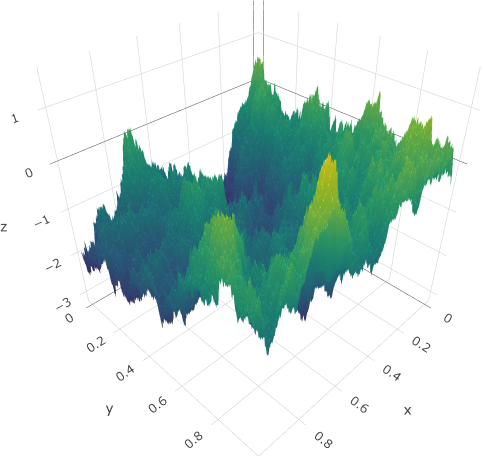
\includegraphics[width=\textwidth]{figures/surface.png}
\caption{A realization of a spatial Gaussian process (left) and an
approximation of that realization over a triangular mesh (right).}
\label{surface}
\end{figure}

\begin{figure}[p]
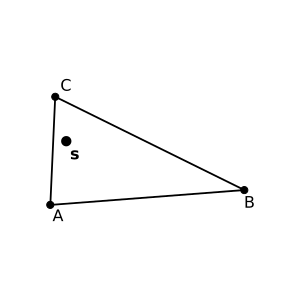
\includegraphics[width=0.5\textwidth]{figures/triangle.png}
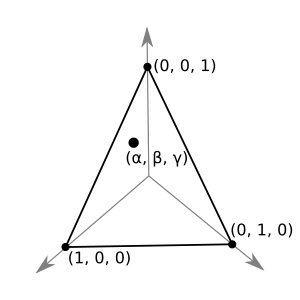
\includegraphics[width=0.5\textwidth]{figures/simplex.png}
\caption{An illustration of the transformation from a mesh triangle to the
simplex. \((\alpha, \beta, \gamma)\) are the barycentric coordinates of
\(\mathbf{s}\)}
\label{surface}
\end{figure}

The SPDE approach is implemented in the \texttt{R-INLA} package along with
tools for constructing triangulation meshes.


\subsection{Going Off the Grid}

Log-likelihood:
\begin{displaymath}
\ell(Z) = C - \int \lambda(\mathbf{s}) d\mathbf{s}
+ \sum \log\left(\lambda(\mathbf{s_{i}})\right)
\end{displaymath}

\cite{simpsonetal}:
$$\ell(Z) \approx C - \sum_{i} \tilde{\alpha}_{i} \exp\left[\sum_{j} z_{j}\phi_{j}(\tilde{\mathbf{s}}_{i})\right] + \sum_{i} \sum_{j} z_{j}\phi_{j}(\mathbf{s_{i}})$$

(Poisson distribution)


\subsection{Variable Sampling Effort}

Observed a thinned process

Thinning process can be known or unknown

Idea has been around a while but most applications have used
gridding~\cite{chakrabortyetal}.

Scale SPDE node integration weights by thinning probabilities when known

Incorporate log-linear model for thinning probability when unknown \cite{yuanetal}


\section{Applications}
%  {\bf Application of your Methodology:} Present some applications of the reviewed methods to some recent data in this or more sections. Also note: Simulation studies can be presented as a sub-section in this section or in a new standalone section.


\subsection{Simulation Study}


\subsection{Data Application}

Examples with data, maybe \texttt{bei} dataset or Victorville


\section{Conclusion and Discussion}
%  {\bf Conclusion and Discussion:} In this conclusion and discussion section, provide conclusions of your review and provide anticipated future direction(s) in this area.


%\section*{Acknowledgement(s)}

%An unnumbered section, e.g.\ \verb"\section*{Acknowledgements}", may be used for thanks, etc.\ if required and included \emph{in the non-anonymous version} before any Notes or References.

%\section*{Disclosure statement}

%An unnumbered section, e.g.\ \verb"\section*{Disclosure statement}", may be used to declare any potential conflict of interest and included \emph{in the non-anonymous version} before any Notes or References, after any Acknowledgements and before any Funding information.

%\section*{Funding}

%An unnumbered section, e.g.\ \verb"\section*{Funding}", may be used for grant details, etc.\ if required and included \emph{in the non-anonymous version} before any Notes or References.

%\section*{Notes on contributor(s)}

%An unnumbered section, e.g.\ \verb"\section*{Notes on contributors}", may be included \emph{in the non-anonymous version} if required. A photograph may be added if requested.

%\section*{Nomenclature/Notation}

%An unnumbered section, e.g.\ \verb"\section*{Nomenclature}" (or \verb"\section*{Notation}"), may be included if required, before any Notes or References.

%\section*{Notes}

%An unnumbered `Notes' section may be included before the References (if using the \verb"endnotes" package, use the command \verb"\theendnotes" where the notes are to appear, instead of creating a \verb"\section*").

\bibliographystyle{tfs}
\bibliography{jas-inla-review}

\end{document}
